%%%%%%%%%%%%%%%%%%%%%%%%%%%%%%%%%%%%%%%%%%%%%%%%%%%%%%%%%%%%
%%%%%%%%%%%          C O P U L A S         %%%%%%%%%%%%%%%%%
%%%%%%%%%%%%%%%%%%%%%%%%%%%%%%%%%%%%%%%%%%%%%%%%%%%%%%%%%%%%

\chapter{Cópulas}\label{CapCopulas}

En este capítulo se definirá el concepto de cópulas, que constituye la herramienta principal para modelar las dependencias entre las covariables. Se hará especial hincapié en las cópulas bivariadas, ya que, dada una función de distribución de un vector aleatorio, esta puede representarse como el producto de cópulas bivariadas condicionales. Esta forma de descomposición se conoce como R-Vines. Sin embargo, esta descomposición no es única, ya que diferentes representaciones pueden obtenerse al permutar el orden de descomposición. En particular, se detallará una forma llamada D-Vine, que se asocia con un grafo o árboles. Utilizando el grafo, es sencillo visualizar las dependencias condicionales o cópulas condicionales necesarias para realizar regresiones utilizando las estructuras mencionadas.

Uno de los principales resultados en los que se basa la teoría de cópulas es el Teorema de Sklar \ref{TeoSklar}. Este teorema proporciona la noción fundamental de las cópulas al establecer una relación entre la función de distribución conjunta de cualquier vector de variables aleatorias y sus distribuciones marginales, que no necesariamente deben ser conocidas. 


\begin{teor}[Teorema de Sklar]\label{TeoSklar}
    \begin{enumerate}
    \item Para cada función de distribución $H$ con distribuciones marginales univariadas $F_1, \dots, F_d$, existe una cópula $C$ $d-dimensional$ tal que 
    \begin{equation}\label{eqsklar}
        H(x) = C(F_1(x_1), F_2(x_2), \dots, F_d(x_d)), \quad x \in \mathbb{R}^{d},
    \end{equation}

    La cópulas C esta únicamente definida en $\prod_{j = 1}^{d}ran F_j$ y esta definida por

    \begin{equation}
        C(u) = H(F_1^{\leftarrow}(u_1), \dots, F_d^{\leftarrow}(u_d)), \quad u \in \prod_{j = 1}^{d}ran F_j
    \end{equation}
    %%%%%%%%%%%%%%%%%%%%%%%%%%%%%%%%%%%%
    
    \item Por el contrario, dada una cópula $C$ $d-dimensional$ y funciones de distribución univariadas $F_1, \dots, F_d$ y$H$ definida como en \eqref{eqsklar}, es una función de distribución $d$ $dimensional$ con marginales $F_1, \dots, F_d$. \cite{CopulasR}
    \end{enumerate}
\end{teor}

El teorema de Sklar establece que cualquier función de distribución conjunta puede descomponerse en sus distribuciones marginales y una cópula. Esto es posible gracias al resultado de la transformación integral de probabilidad \eqref{PITdist}, que indica que cualquier distribución continua puede transformarse en una distribución uniforme estándar. Por lo tanto, una cópula descompone esta distribución conjunta, cuyas marginales pueden ser complejas, en términos de otra función de distribución cuya característica es que sus distribuciones marginales son uniformes en el intervalo $[0,1]$. Esta descomposición permite estudiar la dependencia entre las variables de manera independiente de las distribuciones marginales originales.

Como resumen, dado un vector $X = (X_1, \dots, X_d)$ con funciones de distribución marginal $F_1, \dots, F_d$, existe una cópula $C$ asociada a $X$. Si solo se está interesado en la estructura de dependencia de $X$, se puede considerar la escala $u$ o la escala cópula aplicando la transformación integral de probabilidad a sus marginales $U_j := F_j(X_j), j = 1, \dots, d$.

En conclusión, es importante destacar que las distribuciones marginales de la cópula no contienen información sobre cómo cada variable aleatoria puede interactuar con las demás. Toda la información sobre su dependencia se encuentra en la función de cópula subyacente.

\section{Conceptos Preliminares}

Una copula en palabras generales, es una distribución multivariada con funciones de densidad marginales uniforme estándar, esta es la conexión de las marginales con la distribución conjunta de ahí el nombre de copula. Estas son utilizadas para modelar la dependencia entre múltiples variables las cuales no son necesariamente lineales lo cual permite capturar patrones de correlación no lineal y asimétrica, lo que puede ser útil en la detección de anomalías, la segmentación de datos. Estas pueden ser paramétricas como no paramétricas \cite{CopulasR}.

Además, las cópulas se modelan a través de los datos, lo que permite capturar y modelar de manera precisa las relaciones de dependencia entre las variables. Esto proporciona una herramienta poderosa para analizar y entender las interacciones complejas en conjuntos de datos multivariados.


\begin{defn}[Subcópula]
    Una subcópula 2-dimensional es una función $C'$ con las siguientes propiedades:

    \begin{enumerate}
        \item \textbf{Dominio}: El dominio de la subcópula $C'$ es el producto cartesiano de dos subconjuntos $S_1$ y $S_2$ del intervalo $[0, 1]$, denotado como $S_1 \times S_2$.

        \item \textbf{Aterrizado (Grounded) y 2-creciente}: Grounded quiere decir que, $C(0,v)=0$ y $C(u,0)=0$ para todo $u$ en $u \in S_1$ y $v \in S_2$. 
        $2$-creciente, significa que para cualquier valor fijo de un argumento, aumentar el otro argumento nunca disminuye el valor de $C$.

        \item \textbf{Condición sobre los márgenes}: Para cada $u$ en $S_1$ y $v$ en $S_2$, 
        \begin{equation}
            C'(u, 1) = u, \quad C'(1, v) = v
        \end{equation}

        es decir, cuando se fija uno de los argumentos, la subcópula se comporta como la respectiva distribución marginal
    \end{enumerate}
\end{defn}


\begin{defn}[Cópula 2 dimensional]
    Una cópula bidimensional (o 2-cópula, o simplemente, una cópula) es una 2-subcópula $C$ cuyo dominio es el conjunto $I^2$. Donde $I$ es el intervalo unitario $[0,1]$. 
\end{defn}



\begin{defn}[Subcópula n-dimensional]
    Una subcópula n-dimensional es una función $C'$ con las siguientes propiedades:

    \begin{enumerate}
        \item \textbf{Dominio}: El dominio de la subcópula $C'$ es el producto cartesiano de n subconjuntos $S_i $ para $ i = \left\{ 1, \dots, n\right\}$ del intervalo $[0, 1]$, denotado como $S_1 \times \cdots \times S_n$.

        \item \textbf{Aterrizado (Grounded) y n-creciente}: Grounded quiere decir que, $C(u_1, \dots, u_n)=0$ si alguna $u_i = 0$, para todo $u_1$ en $u_1 \in S_i$. 
        $n$-creciente, significa que para cualquier valor fijo de un argumento, aumentar el otro argumento nunca disminuye el valor de $C$.

        \item \textbf{Condición sobre los márgenes}: Para cada $u_i$ en $S_i$ para $i =  \left\{ 1, \dots, n\right\}$, 
        \begin{equation}
            C'(1, \dots, u_i, \dots,  1) = u_i, \quad \left\{ 1, \dots, n\right\}
        \end{equation}

        es decir, cuando se fija uno de los argumentos, la subcópula se comporta como la respectiva distribución marginal
    \end{enumerate}
\end{defn}

En otras palabras, una cópula es una subcópula bidimensional cuyo dominio abarca todo el cuadrado unitario $[0, 1]^2$. Esto significa que la cópula relaciona las distribuciones marginales de dos variables aleatorias y describe la estructura de dependencia conjunta entre ellas a lo largo de todo el rango posible de valores que pueden tomar \cite{nelsenintroduction}.

\begin{defn}[Cópula n dimensional]
    Una cópula n dimensional es una 2-subcópula $C$ cuyo dominio es el conjunto $I^n$. Donde $I$ es el intervalo unitario $[0,1]$. 
\end{defn}

\begin{ejemplo}[Cópula Producto]
    La cópula más sencilla que se construye consiste en multiplicar las funciones de distribución marginales de las variables aleatorias individuales.

    Sea $X = (X_1, X_2)$ donde cada entrada del vector aleatorio tiene como función de distribución $X_i \sim F(X_i)$, si se define $u_i = F(x_i)$ entonces,

    \begin{equation}
         \prod (u_1, u_2) = u_1 \cdot u_2
    \end{equation}

    es una cópula.

    Esto es claro, ya que cada $u_i \sim U(0, 1)$, haciendo la transformación integral de probabilidad \ref{PITdef} y es función de distribución pues es la definición de variables aleatorias independiente. Cabe mencionar que Si dos variables aleatorias $X$ e $Y$ están relacionadas a través de una cópula independiente, significa que no hay ninguna relación o dependencia entre ellas.
\end{ejemplo}

El requisito de que las distribuciones marginales sean uniformes en el intervalo $[0,1]$ es en cierto sentido arbitrario, ya que las cópulas pueden definirse para cualquier distribución marginal. Sin embargo, trabajar con distribuciones marginales uniformes estándar simplifica los cálculos y la interpretación de las cópulas. El teorema de transformación integral es una herramienta fundamental en el estudio de cópula el cuál simplifica la teoría y las aplicaciones prácticas de las cópulas, lo que hace que trabajar con ellas sea más conveniente y comprensible. \cite{CopulasR}

Con el objetivo de estimar la cópula subyacente a partir de un conjunto de observaciones disponibles. Se propone un ajuste para vectores de variables continuas \cite{CopulasR}.

\begin{defn}[Aproximación Empírica para una Cópula de dim. $2$ ]
    Para una muestra de una copula bivariada $\left\{u_{1 i}, u_{2 i}, i=1, \ldots, n\right\}$, la aproximación empírica de la cópula se define como

    \begin{equation}
        \hat{C}\left(u_1, u_2\right):=\frac{1}{n+1} \sum_{i=1}^n 1_{\left\{u_{1 i} \leq u_1, u_{2 i} \leq u_2\right\}} \text { para todo } 0 \leq u_1, u_2 \leq 1.
    \end{equation}
\end{defn}

%%%%%%%%%%%%%%%%%%%%%%%%%%%%%%%%%%%%%%%%%%%%%%%%%%%%%%%%
%%%%% C O P U L A S  D - D I M E N S I O N A L E S %%%%%
%%%%%%%%%%%%%%%%%%%%%%%%%%%%%%%%%%%%%%%%%%%%%%%%%%%%%%%%

Ahora, se generaliza para $d$ dimensiones. Se enfatizó en 2 dimensiones ya que estas constituirán nuestras herramientas principales en el modelado. Para que una función $C: [0, 1]^d \to [0, 1]$ sea considerada una cópula, es necesario que cumpla con ciertas propiedades que garanticen que $C$ sea una función de distribución multivariada. Para lograr esto, se introducirán conceptos adicionales estos son principalmente tomados de \cite{nelsenintroduction} y \cite{TesisEmanuel}.

\begin{defn}
    Para cualquier $a, b \in [0, 1]$, tal que $a \leq b$, se denota al hiperectángulo $(a, b]$, está definido por $\left\{ u \in [0, 1]^{d}: a <u \leq b\right\}$.
\end{defn}

\begin{defn}
    Para cualquier hiperectángulo $(a, b] \in [0, 1]^d$, se define el $C-volumen$ como
    \begin{equation}
        \Delta_{(\boldsymbol{a}, \boldsymbol{b}]} C=\sum_{\boldsymbol{i} \in\{0,1\}^d}(-1)^{\sum_{j=1}^d i_j} C\left(a_1^{i_1} b_1^{1-i_1}, \ldots, a_d^{i_d} b_d^{1-i_d}\right),
    \end{equation}
\end{defn}

Si todos los hiperectángulos $(a, b] \in [0, 1]^d$ es no negativo, es decir, 

\begin{equation}
    \Delta_{(\boldsymbol{a}, \boldsymbol{b}]} C \geq 0 \quad \text { for all } a, b \in[0,1]^d, a \leq b
\end{equation}

Una copula se dice absolutamente continua si la copula $C$ admite función de densidad. Por otro lado, el Teorema de Sklar \ref{TeoSklar} es el teorema central de copulas; este explica por qué las cópulas determinan la dependencia entre los componentes de un vector aleatorio.


%%%%%%%%%%%%%%%%%%%%%%%%%%%%%%%%%%%%%%%%%%%%%%%%%%%%%%
%%%%%%%%% C O T A S  D E  F R E C H 
%%%%%%%%%%%%%%%%%%%%%%%%%%%%%%%%%%%%%%%%%%%%%%%%%%%%%%

\subsection{Cotas de Frechet-Hoeffding}

Las cotas proporcionan una forma rápida y sencilla de verificar si una función dada $C(u, v)$  es una cópula válida. Es decir, si una función no cumple con las cotas de Fréchet-Hoeffding, entonces no puede ser considerada una cópula. Adicionalmente, al utilizar cópulas en el análisis de datos, las cotas pueden proporcionar información útil sobre la naturaleza de la dependencia entre variables. Por ejemplo, si una cópula está cerca de las cotas inferiores, sugiere una fuerte dependencia negativa, mientras que si está cerca de las cotas superiores, sugiere una fuerte dependencia positiva.

\begin{defn}[Cotas de Fréchet-Hoeffding]
    Sea $C$ una cópula d-dimensional. Entonces para toda $\boldsymbol{u} \in[0,1]^d$,

    \begin{equation}
        W^d(\boldsymbol{u}) \leq C(\boldsymbol{u}) \leq M^d(\boldsymbol{u}),
    \end{equation}

Donde $W^d(\boldsymbol{u}):= \max \left(u_1+\ldots+u_d-d+1,0\right)$ y $M^d(\boldsymbol{u}):=\min \left(u_1, \ldots, u_d\right)$.
\end{defn}

Se puede demostrar que el límite superior $M^d$ es una cópula, mientras que el límite inferior $W^d$ es una cópula sólo para $d = 2$.

Estas cotas son importantes en la teoría de las copulas porque proporcionan una referencia útil para evaluar la dependencia entre las variables aleatorias como la enuncia en Lema \ref{lemCotas}. Además, pueden ser utilizadas para verificar la validez de un modelo de copula propuesto y para evaluar la bondad de ajuste de una copula a un conjunto de datos observados.

\begin{lema}\label{lemCotas}
    Sean $X$ e $Y$ variables aleatorias con función de distribución conjunta $H$. Entonces, $H$ es igual a su límite superior de Fréchet-Hoeffding si y solo si para cada $(x, y)$ en $\mathbb{R}^2$, ya sea que $P[X > x, Y \leq y] = 0$ o que $P[X \leq x, Y > y] = 0$.
\end{lema}

\begin{teor}
    Se dice que $X$ e $Y$ son variables aleatorias con función de distribución conjunta $H$. Entonces, $H$ es idénticamente igual a su límite superior de Fréchet-Hoeffding si y solo si el soporte de $H$ es un subconjunto no decreciente de $\mathbb{R}^2$.
\end{teor}

\begin{teor}
    Se dice que $X$ e $Y$ son variables aleatorias con función de distribución conjunta $H$. Entonces, $H$ es idénticamente igual a su límite inferior de Fréchet-Hoeffding si y solo si el soporte de $H$ es un subconjunto no creciente de $\mathbb{R}^2$.
\end{teor}

\begin{defn}
    Sean $X$, $Y$ variables aleatorias continuas con cópula subyacente $C_{XY}$, entonces $X$, $Y$ guardan una dependencia
    estrictamente monótona si 
    
    \begin{equation}
        C_{XY}(u, v) - \Pi(u, v) > 0 \textit{ o } C_{XY}(u, v) - \Pi(u, v) < 0, \forall u, v \in I
    \end{equation}
    
    Nótese que los extremos de la dependencia estrictamente monótona son las cópulas $M$ y $W$. \cite[pág 42]{TesisEmanuel}
\end{defn}


Los lemas y teoremas anteriores proporcionan condiciones sobre la función de distribución que ayudan a comprender la naturaleza de la relación entre las variables $X$ e $Y$, donde una variable tiende a moverse en una sola dirección a medida que la otra cambia. Esto se refiere a si la dependencia entre las variables es monótona. Además, estos resultados establecen criterios que pueden guiar la elección de modelos probabilísticos adecuados para describir la relación entre dos variables aleatorias.
%%%%%%%%%%%%%%%%%%%%%%%%%%%%%%%%%%%%%%%%%%%%%%%%%%%%%
%%%%%%%%%%%%%%% Medidas de Dependencia %%%%%%%%%%%%%%
%%%%%%%%%%%%%%%%%%%%%%%%%%%%%%%%%%%%%%%%%%%%%%%%%%%%%

\section{Medidas de Dependencia}

Existen diversas medidas que se encargan de cuantificar la fuerza y dirección en la que dos variables aleatorias se relacionan. Estas medidas son fundamentales en el análisis de dependencia entre variables, ya que permiten comprender cómo cambia una variable en respuesta a cambios en otra. 

Entre las más comunes se encuentra el coeficiente de correlación de Pearson, que mide la relación lineal entre dos variables. Sin embargo, en muchos casos, las relaciones entre variables pueden no ser lineales o pueden presentar patrones más complejos. Es ahí donde entran en juego medidas alternativas como el coeficiente de correlación de Kendall y el coeficiente de correlación de Spearman. Estas medidas, también conocidas como correlaciones de rango, evalúan la asociación entre variables basándose en el ordenamiento de los datos en lugar de en sus valores exactos. \cite{czadoAnalyzing}



%%%%%%%%%%%%%%%%%%%%%%%%%%%%%%%%%%%%%%%%%%%%%%%%%%%%%%%%%%%%%%%
\subsubsection{Correlación de Pearson}

Se utilizó el coeficiente de Pearson para medir la correlación lineal entre dos variables aleatorias. En la Ecuación \eqref{correlacion} se muestra como se define el coeficiente de Pearson para dos variables aleatorias $X$ y $Y$. Cuando se quiere medir el coeficiente de correlación entre dos muestras se define el coeficiente de correlación de Pearson muestral como en la Ecuación \eqref{corrMuestral}.

\begin{equation}\label{correlacion}
    \rho_{X, Y} = \frac{Cov(X, Y)}{\sqrt{Var(X) \cdot Var(Y)}} = \frac{\sigma_{X, Y}}{\sigma_X \sigma_Y}
\end{equation}

\begin{equation}\label{corrMuestral}
    r_{x y}=\frac{\sum_{i=1}^n\left(x_i-\bar{x}\right)\left(y_i-\bar{y}\right)}{\sqrt{\sum_{i=1}^n\left(x_i-\bar{x}\right)^2} \sqrt{\sum_{i=1}^n\left(y_i-\bar{y}\right)^2}}
\end{equation}

 Una propiedad distintiva de este coeficiente es que se encuentra acotado entre $-1$ y $1$. Si este coeficiente muy cercano a $1$ en valor absoluto entonces se existe una fuerte dependencia lineal puede ser una dependencia proporcional o inversamente proporcional dependiendo si el signo del coeficiente es positivo o negativo respectivamente. Por otro lado, si este coeficiente es muy cercano a 0 entonces la dependencia lineal entre estas dos variables es muy baja. Cabe destacar que si este coeficiente es 0 o muy cercano a 0 no implica que no existe alguna dependencia entre las dos variables solamente indica que no es lineal.

Como se ha mencionado previamente, el coeficiente de correlación lineal no proporciona información relevante cuando las variables no exhiben una relación lineal, y además es susceptible a ser influenciado por valores atípicos. Con el propósito de entender y visualizar las relaciones entre variables de manera más completa, se introducirán otras medidas de dependencia que se basan en la concordancia, es decir, en la consistencia en la dirección de los cambios entre las variables.



%%%%%%%%%%%%%%%%%%%%%%%%%%%%%%%%%%%%%%%%%%%%%%%
%%%%%%%%%  C O N C O O R D A N C I A %%%%%%%%%% 
%%%%%%%%%%%%%%%%%%%%%%%%%%%%%%%%%%%%%%%%%%%%%%%

\subsection{Concoordancia}

Existen varios aspectos de interés en una medida de dependencia entre variables aleatorias, siendo la `invarianza ante la escala' uno de los más destacados. Esto implica que la medida no cambia bajo transformaciones estrictamente crecientes. Como se mencionó anteriormente, las copulas son transformaciones crecientes que describen la relación de la distribución conjunta de variables aleatorias. Por lo tanto, este tipo de medidas son de gran utilidad. Entre las medidas más famosas invariantes ante la escala se encuentran la $\tau$ de Kendall y la $\rho$ de Spearman.\cite{czadoAnalyzing}

La concordancia y la monotonía están estrechamente relacionadas porque la concordancia es una forma de medir cuán consistentemente dos variables mantienen una relación monótona. Una medida de concordancia, en términos simples, evalúa cuán fuertemente están asociados los valores de una variable con los valores altos o bajos de la otra variable. Más precisamente, si $(x_i, y_i)$ y $(x_j, y_j)$ denoten dos observaciones de un vector $(X, Y)$ de variables aleatorias continuas. 

\begin{defn}[Concoordancia]
    Se dice que $(x_i, y_i)$ y $(x_j, y_j)$ son concordantes si $x_i < x_j$ y $y_i < y_j$. De manera similar, se dice que $(x_i, y_i)$ y $(x_j, y_j)$ son discordantes si $x_i < x_j$ y $y_i > y_j$, o $si x_i > x_j$ y $y_i < y_j$. 
    
    Alternativamente, $(x_i, y_i)$ y $(x_j, y_j)$ son concordantes si $(x_i - x_j)(y_i - y_j) < 0$.
\end{defn}

Para evaluar y comparar la dependencia entre variables observada en datos reales con la dependencia que se esperaría si las variables fueran independientes, se recurre a la cópula producto. Esta cópula proporciona una referencia fundamental para entender la estructura de dependencia entre variables. Se utiliza la métrica $\mathcal{L}_p$ (ver Definición \ref{lp}), para cuantificar y comparar la discrepancia entre la dependencia observada y la independencia teórica \cite{TesisEmanuel}.

\begin{defn}\label{lp}
    Para cualquier $p \in[1, \infty)$ la distancia $L_p$ entre una cópula $\mathcal{C}$ y $\Pi$ esta dada por:

    \begin{equation}\label{eqLP}
        \mathcal{V}_p(C)=\left(k_p \iint_{\mathcal{I}^2}|\mathcal{C}(u, v)-u v|^p d u d v\right)^{\frac{1}{p}},
    \end{equation}

    donde $k_p$ es una constante elegida de tal modo que, en la Ecuación \eqref{eqLP}, sea igual a $1$ cuando $\mathcal{C}=\mathcal{M}$ o $\mathcal{W}$.
\end{defn}


A continuación, se describen un conjunto mínimo de propiedades deseables para una medida de dependencia no paramétrica. 

\begin{defn}[Medida de Dependencia]
    Una medida numérica $\delta$ de asociación entre dos variables aleatorias continuas X e Y cuya copula es C es una medida de dependencia si satisface las siguientes propiedades (donde se escribe $\delta_{X,Y}$, o $\delta_C$ si es conveniente):

    \begin{enumerate}
        \item $\delta$ está definida para cada par de variables aleatorias continuas X e Y.
        \item $\delta_{X,Y} = \delta_{Y,X}$.
        \item $0 \leq \delta_ {X,Y} \leq 1$.
        \item  $\delta_{X,Y} = 0$ si y solo si $X$ e $Y$ son independientes, $\delta_{X,Y} = 1$ si y solo si cada una de $X$ e $Y$ es casi seguramente una función estrictamente monótona de la otra.
        \item si $\alpha$ y $\beta$ son funciones casi seguramente estrictamente monótonas en $RanX$ y $RanY$, respectivamente, entonces da $\delta_{\alpha(X), \beta(Y)} = \delta_{X,Y}$.
        \item si $\left\{ ( Xn ,Yn )\right\}$ es una secuencia de variables aleatorias continuas con copulas $C_n$, y si $\left\{ C_n\right\}$ converge punto a punto a $C$, entonces $\lim_{n \to \infty} \delta C_n = \delta_C$.
    \end{enumerate}
\end{defn}

\begin{defn}
    Una medida numérica $\kappa$ de asociación entre dos variables aleatorias continuas $X$ e $Y$ cuya copula es $C$, es una medida de concordancia si satisface las siguientes propiedades (donde se escribe $\kappa_{X,Y}$ o $\kappa_{C}$ si es conveniente):

    \begin{enumerate}
        \item $-1 \leq \kappa_{X,Y} \leq 1, \kappa_{X,X} = 1, \kappa_{X,-X} = -1$

        \item $\kappa_{X,Y} = \kappa_{Y,X}$

        \item Si $X$ y $Y$ son independientes entonces $\kappa_{X,Y} = 0$.

        \item $\kappa_{-X,Y} = \kappa_{X,-Y} = -\kappa X,Y$
        \item Si $C1 \leq C2$ entonces $\kappa C1 \leq \kappa C2$
    \end{enumerate}
\end{defn}
%%%%%%%%%%%%%%%%%%%%%%%%%%%%%%%%%%%%%%%%%%%%%%%%%%%%%%%
\subsubsection{$\rho$ de Spearman}

El coeficiente de correlación de Sperman el cuál evalúa la relación monotónica entre dos variables, no asume una relación lineal y es robusta ante la presencia a valores atípico, este es definida como se muestra en la ecuación \eqref{corSpear}.  

\begin{equation}\label{corSpear}
    r_s=\rho_{\mathrm{R}(X), \mathrm{R}(Y)}=\frac{\operatorname{cov}(\mathrm{R}(X), \mathrm{R}(Y))}{\sigma_{\mathrm{R}(X)} \sigma_{\mathrm{R}(Y)}}
\end{equation}

Donde $\rho$ denota el coeficiente de correlación de Pearson, $\mathrm{R}(X)$ y $\mathrm{R}(Y)$, el rango de la variable aleatoria $X$ y $Y$ respectivamente y $\sigma_{\mathrm{R}(X)}$ y $\sigma_{\mathrm{R}(Y)}$ la desviación estándar del rango de las variables $X$ y $Y$ respectivamente. En palabras sencillas, el coeficiente de correlación de Spearman es el resultado de aplicar la correlación de Pearson al rango de las variables. Sin embargo, esta puede ser reescrita en términos de dos variables aleatorias $U$ y $V$, y $C$ su respectiva copula asociada como se aprecia en la Ecuación \eqref{SpearTeo}.


\begin{equation}\label{SpearTeo}
    \rho_{\mathbf{C}}=12 \iint_{\mathcal{I}^2} (\mathbf{C}(u, v)-u v) \mathrm{d} u \mathrm{~d} v
\end{equation}

La fórmula empírica para dos vectores muestrales, es la que se muestra en la ecuación \eqref{SWEemp}, donde $\hat{\sigma}_{\mathbf{C}}$ es la cópula empírica. 

\begin{equation}\label{Spearemp}
    \hat{\sigma}_{\mathbf{C}}=\frac{12}{n^2-1} \sum_{i=1}^n \sum_{j=1}^n\hat{\mathbf{C}}_n\left(\frac{i}{n}, \frac{j}{n}\right)-\frac{i}{n} \times \frac{j}{n}
\end{equation}
%%%%%%%%%%%%%%%%%%%%%%%%%%%%%%%%%%%%%
\subsubsection{$\sigma$ de Schweizer y Wolff}

Una medida dependencia adicional la Sigma de Schweizer y Wolff fue propuesta por los matemáticos Peter Schweizer y Ekkehard Wolff. Se utiliza en el contexto de teoría de la copula para cuantificar la asociación entre variables aleatorias de manera más general que las medidas tradicionales de correlación. Esta es definida como en la ecuación \eqref{SWETeo}, donde $C$ es una cópula cuyas marginales son $U$ y $V$.

Es una medida robusta que puede capturar una amplia gama de estructuras de dependencia, incluidas aquellas que son no lineales o no monótonas. 

\begin{equation}\label{SWETeo}
    \sigma_{\mathbf{C}}=12 \iint_{\mathcal{I}^2}|\mathbf{C}(u, v)-u v| \mathrm{d} u \mathrm{~d} v
\end{equation}

La fórmula empírica para dos vectores muestrales, es la que se muestra en la ecuación \eqref{SWEemp}, donde $\hat{\sigma}_{\mathbf{C}}$ es la cópula empírica. Todas las correlaciones anteriormente mencionadas ya están implementadas en el lenguaje de programación R.

\begin{equation}\label{SWEemp}
    \hat{\sigma}_{\mathbf{C}}=\frac{12}{n^2-1} \sum_{i=1}^n \sum_{j=1}^n\left|\hat{\mathbf{C}}_n\left(\frac{i}{n}, \frac{j}{n}\right)-\frac{i}{n} \times \frac{j}{n}\right|
\end{equation}


\begin{propo}
    Sean $X$, $Y$ variables aleatorias con dependencia estrictamente monótona y sea $C$ la cópula asociada. Dadas las medidas de asociación $\rho_C$ de Spearman \eqref{SpearTeo} y $\sigma_C$ de Schweizer y Wolff \eqref{SWETeo}, entonces $|\rho_C| = \sigma_C$
\end{propo}

La proposición anterior ofrece un punto de referencia crucial para evaluar la monotonía de la cópula subyacente $C$ de las variables $X$ y $Y$, utilizando medidas de dependencia. En términos simples, sugiere que cuanto menor sea la diferencia la $\rho$ de Spearman y la $sigma$ de Schweizer y Wolff, mayor será la relación de monotonía entre las variables.

La relevancia de que un par de variables aleatorias mantenga una dependencia estrictamente monótona radica en el hecho de que la mayoría de las cópulas conocidas cumplen con esta condición. Por lo tanto, al buscar un ajuste paramétrico conjunto para un par de variables aleatorias, es crucial identificar dependencias estrictamente monótonas en la muestra que puedan ser modeladas por cópulas bien establecidas. Esto asegura que el modelo propuesto se ajuste de manera precisa a la estructura de dependencia observada en los datos, lo que a su vez mejora la capacidad del modelo para realizar predicciones precisas. \cite[pág. 43]{TesisEmanuel}


%%%%%%%%%%%%%%%%%%%%%%%%%%%%%%%%%%%%%%%%%%%%%%%%
%%%%%%%%%%% L A  D I A G O N A L %%%%%%%%%%%%%%%
%%%%%%%%%%%%%%%%%%%%%%%%%%%%%%%%%%%%%%%%%%%%%%%%

\subsection{La Diagonal}

Durante el proceso de ajuste de modelos probabilísticos, es crucial contar con herramientas que nos permitan comprender las relaciones entre las variables aleatorias. Entre estas herramientas, las secciones diagonal, horizontal y vertical de una cópula juegan un papel fundamental al proporcionar información detallada sobre la estructura de dependencia entre estas variables. A continuación, se da la definición de cada una de ellas. Para demostraciones detalladas ver el libro `\textit{An Introduction to Copulas}' \cite{nelsenintroduction} o la tesis de licenciatura `\textit{Desarrollo Humano e Intensidad Migratoria: Modelado Conjunto Vía Cópulas}'.

\begin{defn}
    Sea $C$ una cópula, y sea $a$ cualquier número en $I$. 
    \begin{enumerate}
        \item La sección horizontal de $C$ en $a$ es una función de $I \to I$ dada por $ t \mapsto C(t, a)$. 
        \item La sección vertical de $C$ en $a$ es una función de $I \to I$ dada por $ t \mapsto C(a, t)$.
        \item La sección diagonal de $C$ es la función $\delta_C$ de $I \to I$ definida por $\delta_C(t) = C(t,t)$.
    \end{enumerate}
\end{defn}

\begin{corl}
    Las secciones horizontal, vertical y diagonal son no decrecientes y uniformemente continuas.
\end{corl}

\begin{figure}[H]
    \centering
    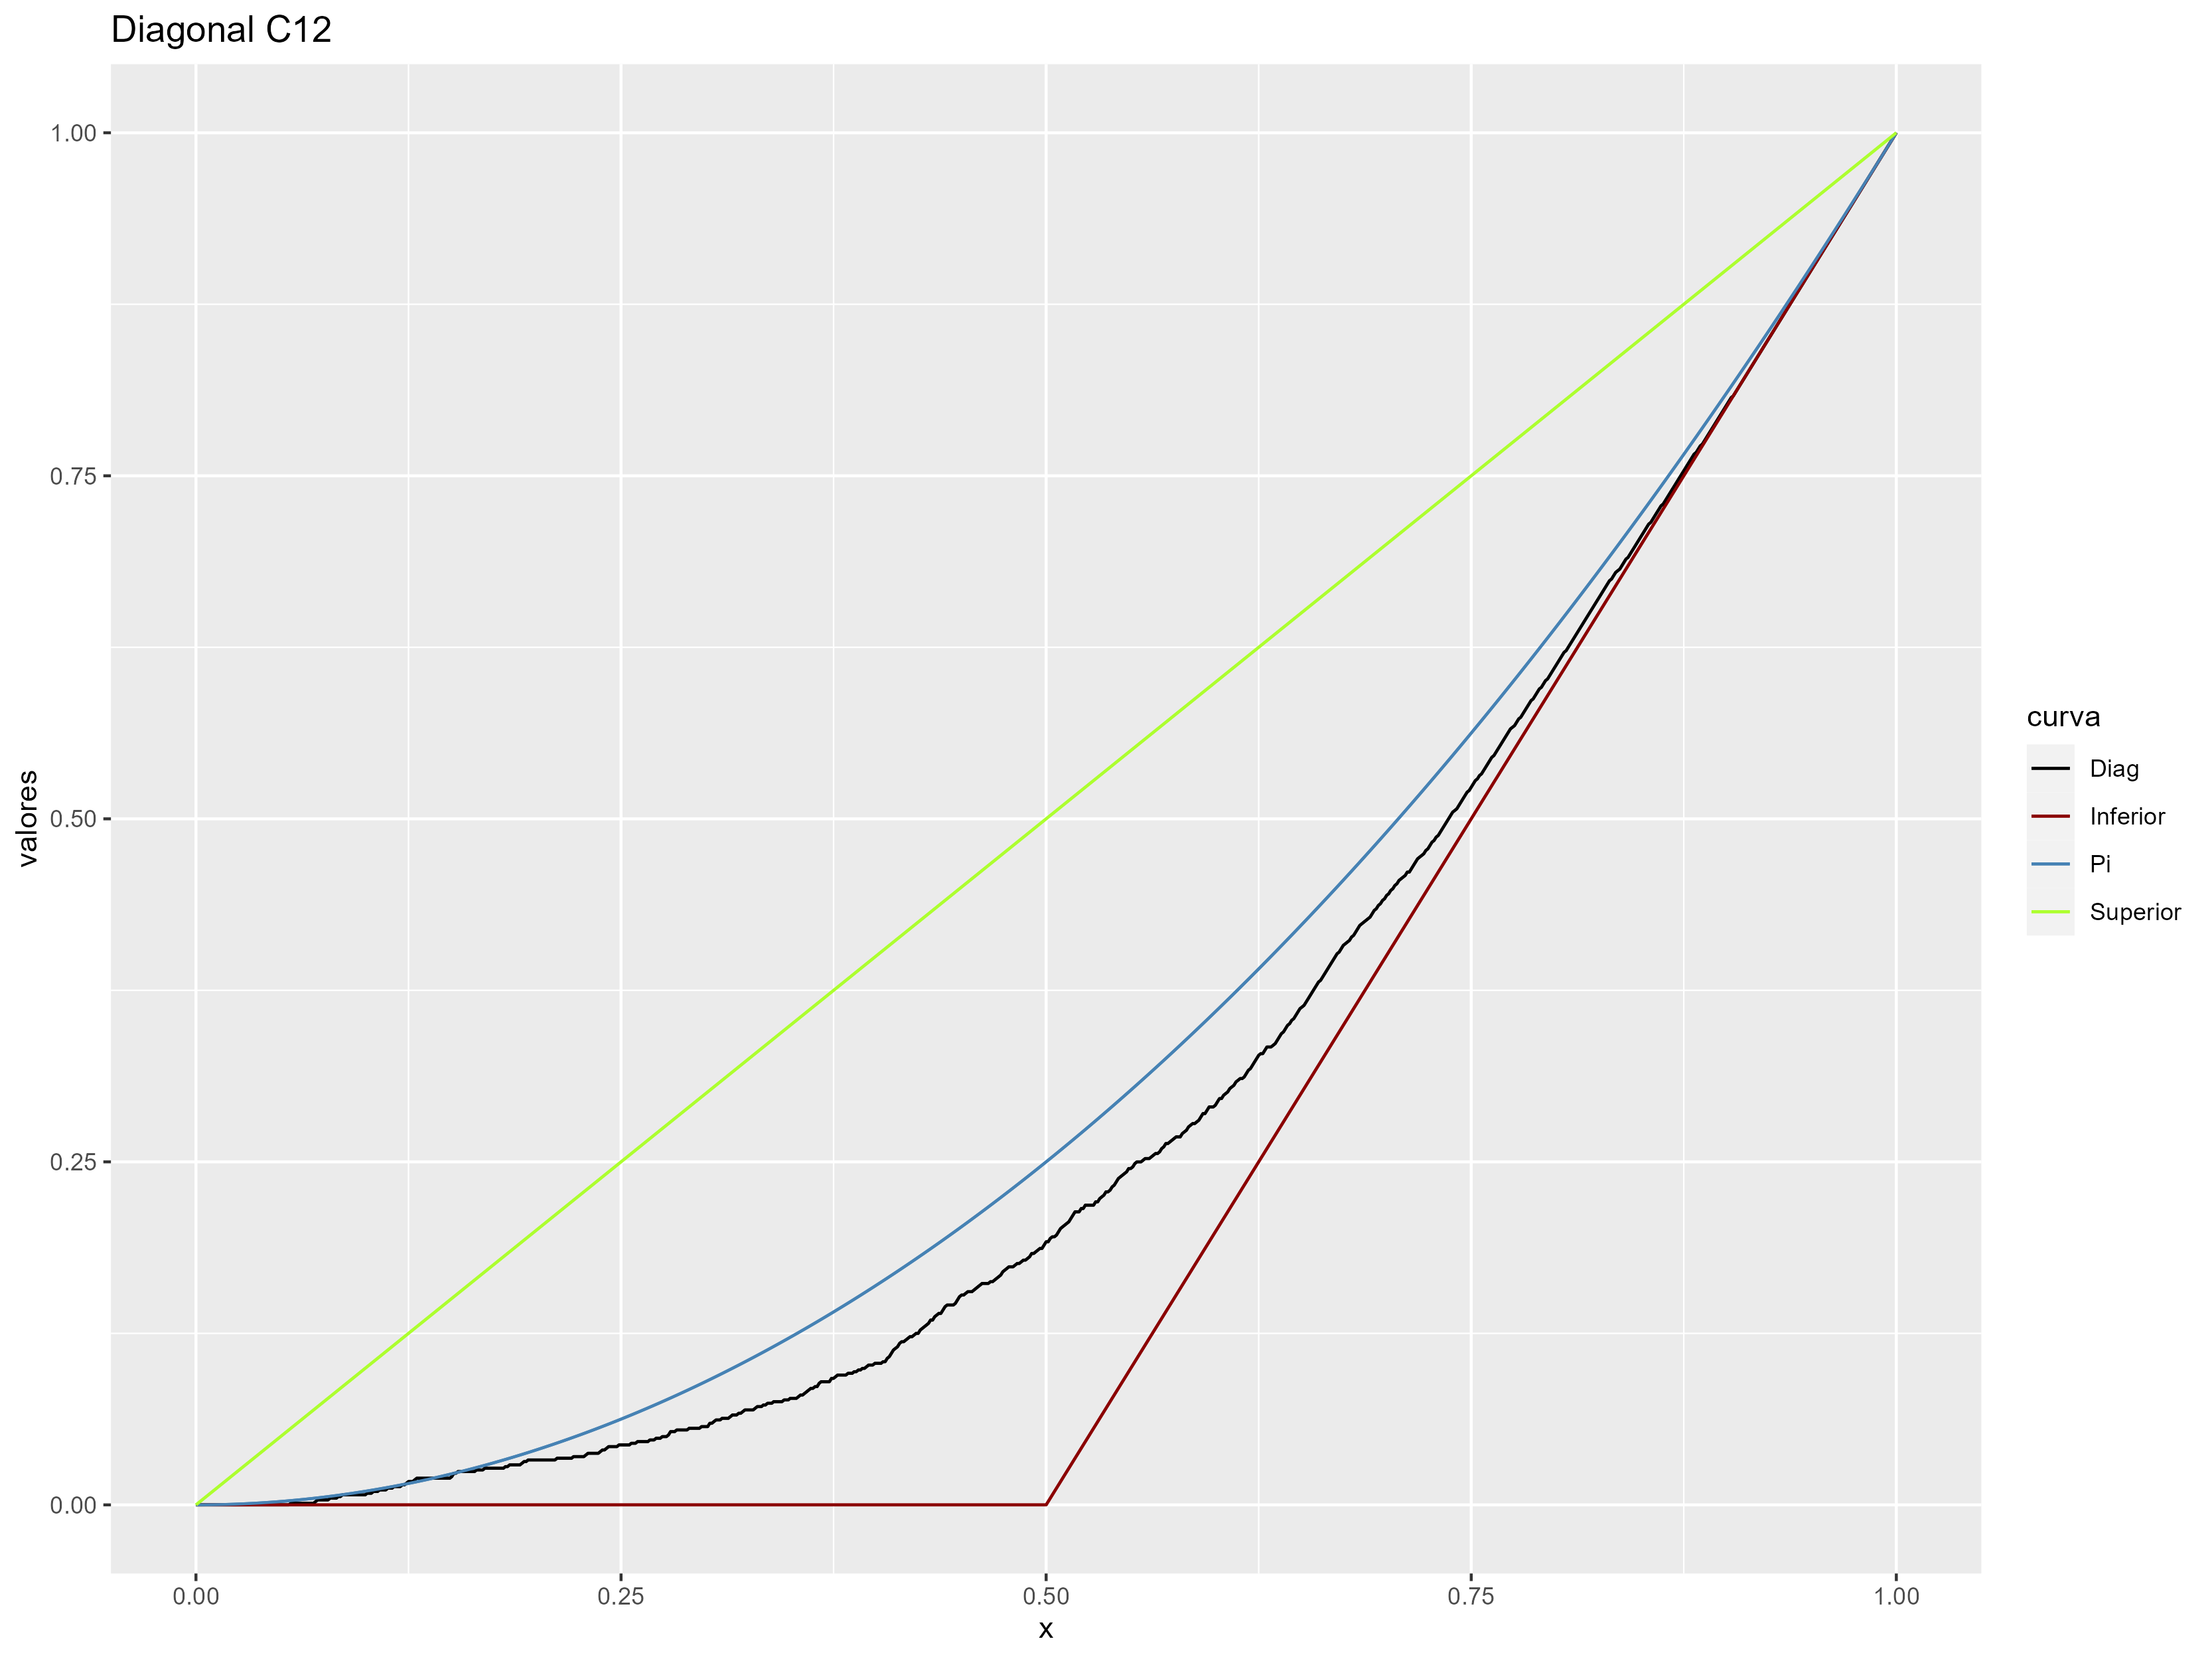
\includegraphics[width =  0.6 \textwidth]{4img/DiagMujC12.png}
    \caption{Ejemplo de la visualización de las diagonales.}
    \label{fig:diagEj}
\end{figure}

Si la cópula es monótona a lo largo de la diagonal, significa que la asociación entre las variables aumenta o disminuye de manera constante a medida que ambas variables aumentan o disminuyen en valor. Esto indica una relación de dependencia monótona entre las variables. \cite{TesisEmanuel}

Para ilustrar cómo se interpretan las diagonales de las cópulas, en la Figura \ref{fig:diagEj}, se muestran varias diagonales de referencia: en azul, la diagonal de la cópula producto o independiente; en verde, la diagonal de la cópula $M$, que es la cota superior; y en rojo, la diagonal de la cópula $W$, que es la cota inferior. En negro se muestra la diagonal de la cópula empírica. Las tres primeras diagonales sirven como referencias para inferir la relación que representa la cópula empírica.

\begin{itemize}
    \item Si la diagonal de la cópula empírica es muy cercana a la diagonal de la cópula independiente, es muy probable que no pase el test de independencia. En caso de que solo una sección de la diagonal de la cópula empírica sea cercana a la de la cópula independiente, se debería considerar la posibilidad de modelar esta relación utilizando una combinación de cópulas. Es decir, una sección se modelaría como una estructura independiente y la otra sección con una cópula diferente.

    \item Por otra parte, si la diagonal de la cópula empírica se encuentra por encima o por debajo de la diagonal de la cópula independiente, esto proporciona información sobre la naturaleza de la relación de monotonía entre las variables. Si está por encima, indica una relación monótona creciente, mientras que si está por debajo, sugiere una relación monótona decreciente. Del mismo modo, esta interpretación puede aplicarse a secciones específicas de la cópula.
\end{itemize}

En la Figura \ref{fig:diagEj}, se puede observar una cópula cuya relación es monótona decreciente en todo el dominio. Además, parece haber secciones donde se encuentra muy cerca de la cópula independiente en los extremos. La noción de cercanía es meramente intuitiva, por lo que este análisis es una herramienta de carácter exploratorio.

Estudiar las secciones diagonal, horizontal y vertical de una cópula en términos de relaciones monótonas, ayuda comprender mejor la dirección y la fuerza de la dependencia entre las variables aleatorias en diferentes escenarios. 



%%%%%%%%%%%%%%%%%%%%%%%%%%%%%%%%%%%%%%%%%%%%%%%%%%%%%
%%%%%%%%%%%%% pares de Copulas %%%%%%%%%%%%%%%%%%%%%%

\section{Cópulas Paramétricas}

Hay variables aleatorias paramétricas, como las distribuciones normales o gamma, poseen una forma específica definida por sus parámetros, lo que facilita su modelado y análisis en diferentes contextos. De manera similar, en el ámbito de las copulas, las copulas paramétricas ofrecen una herramienta poderosa para 
representar la estructura de dependencia entre variables aleatorias. Al ajustar los parámetros de la copula, es posible capturar una amplia gama de patrones de dependencia, desde la independencia hasta la dependencia extrema. 

Este enfoque paramétrico proporciona flexibilidad en la modelización de relaciones complejas entre variables, lo que resulta especialmente útil. En la modelización de variables aleatorias individuales como en la descripción de su dependencia conjunta, el uso de funciones paramétricas es de gran útilidad para capturar con precisión la variabilidad y las interacciones en los datos. En la Figura \ref{fig:Parametric}\footnote{Figura tomada de \cite{ImgCopulas}} se muestran las curvas de nivel de algunas cópulas paramétricas.

\begin{figure}[H]
    \centering
    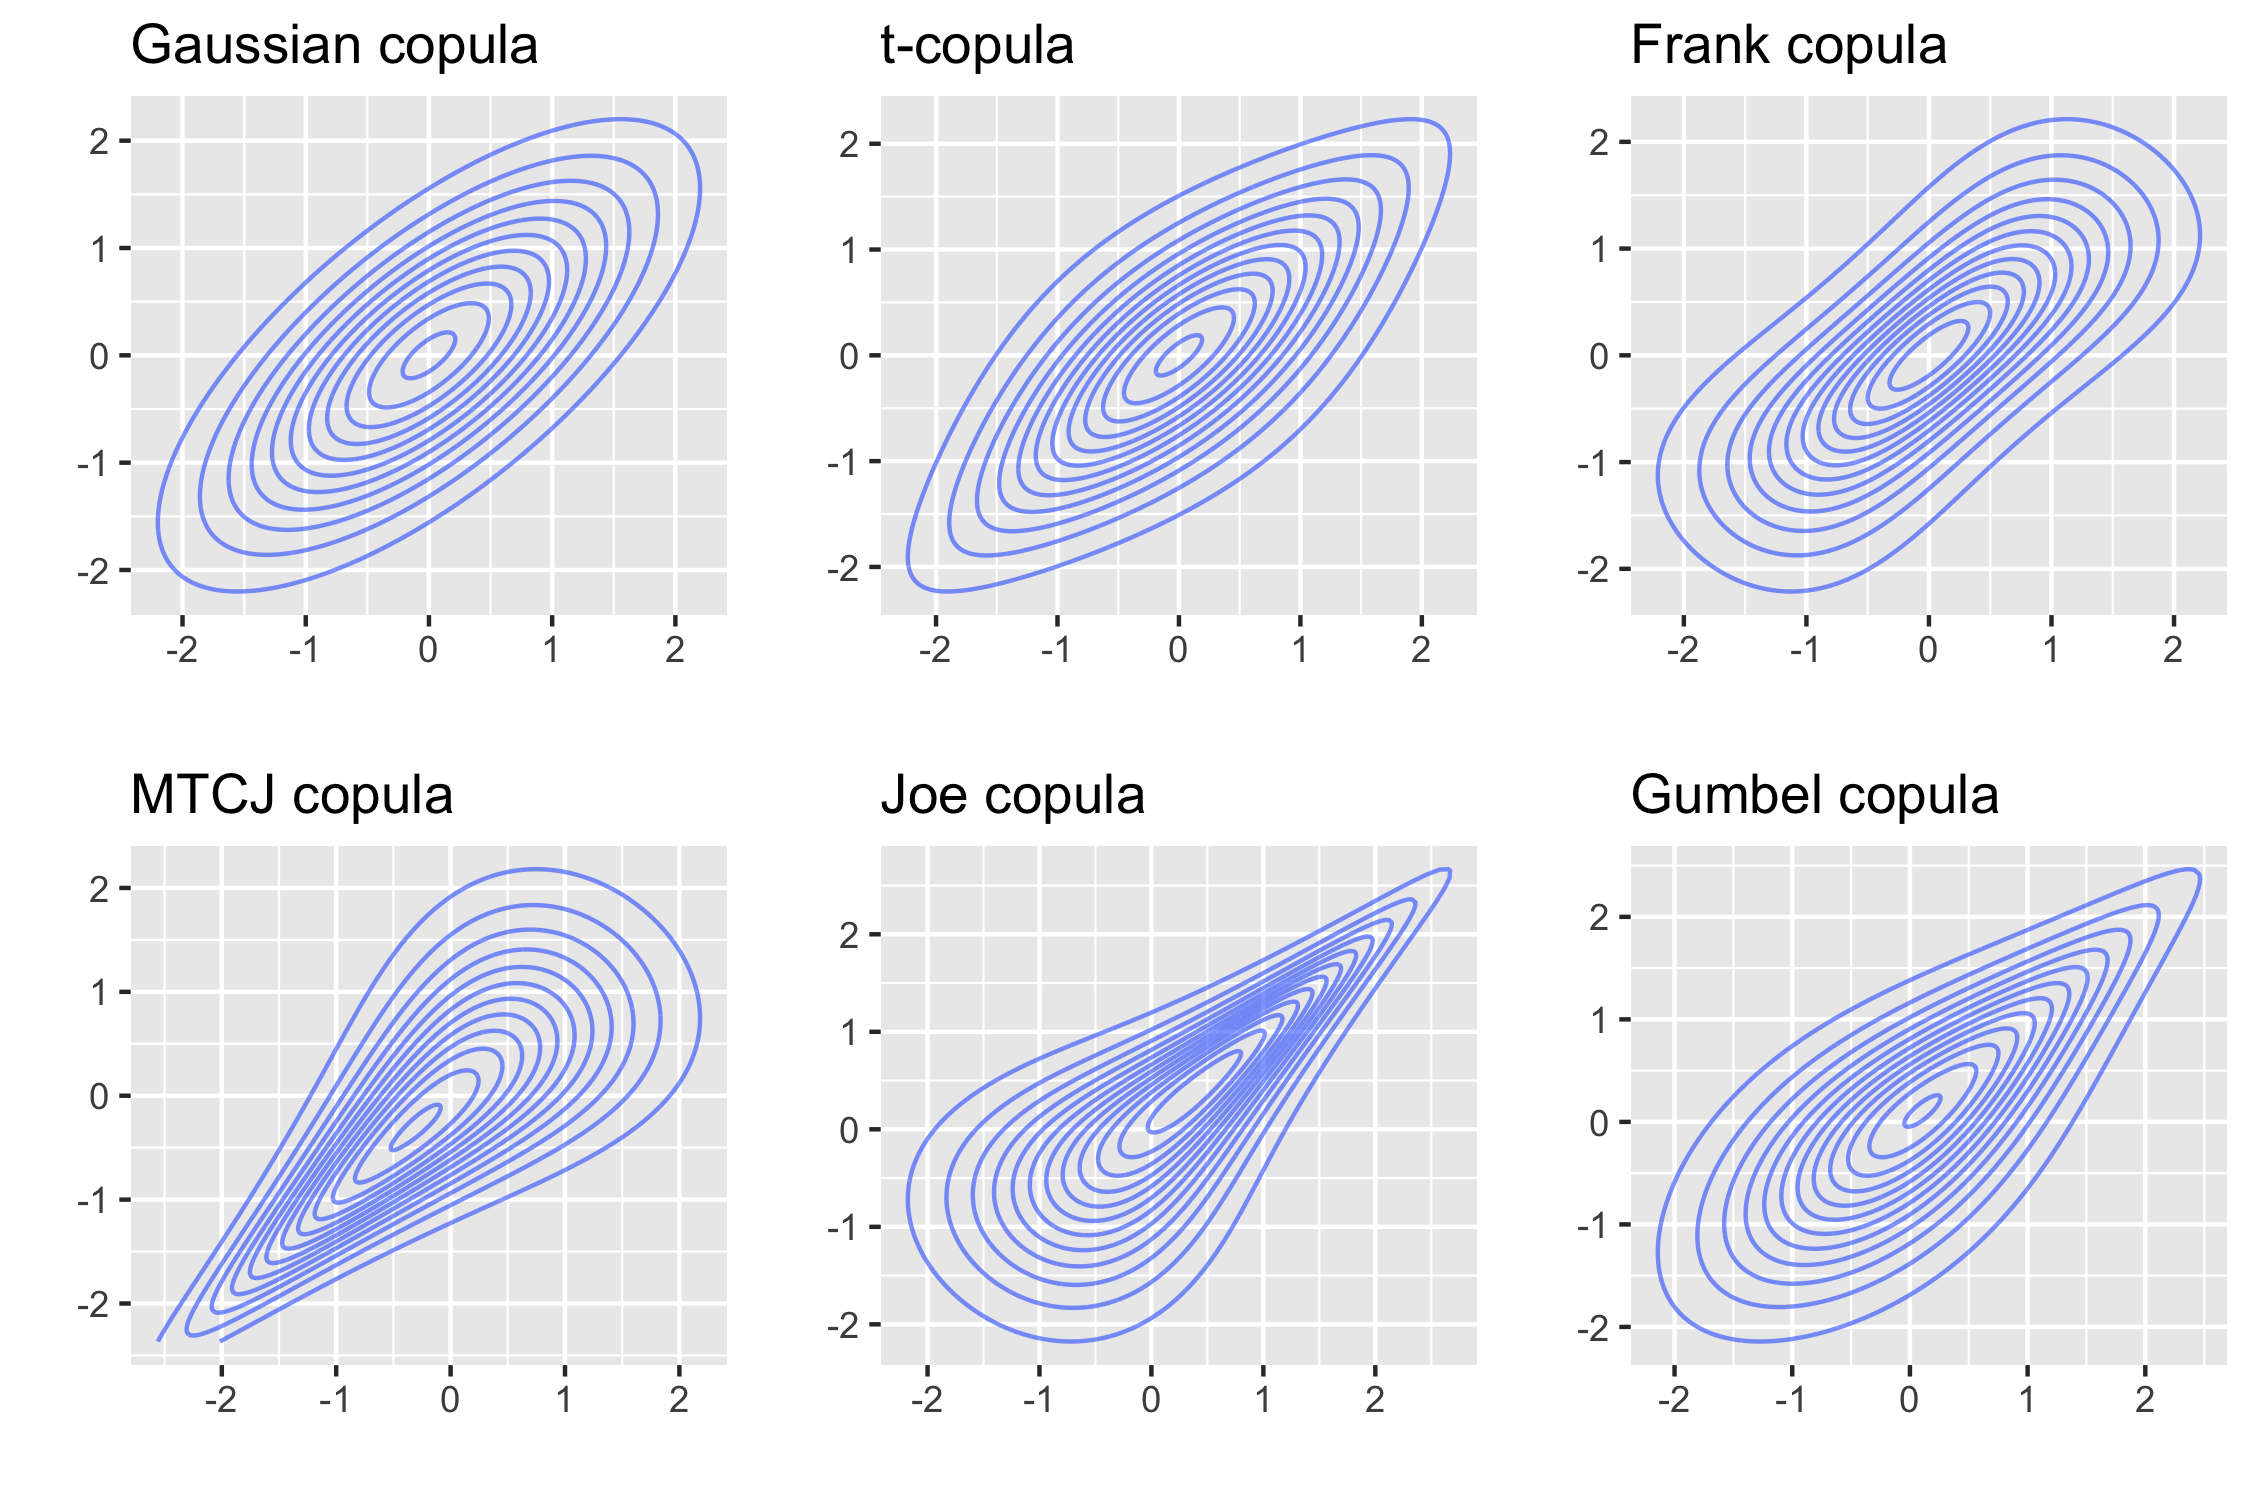
\includegraphics[width = 0.7 \textwidth]{Imagenes/parametricCopulas.png}
    \caption{Ejemplos de cópulas paramétricas.}
    \label{fig:Parametric}
\end{figure}

\begin{ejemplo}[Distribución éstandar Bivariada $t$ de Student] La Distribución éstandar Bivariada $t$ de Student, cuyo vector de media $\boldsymbol{\mu}$ es igual a cero, y la matriz de parámetros de escala es

\begin{equation}
    \Sigma_\rho=\left[\begin{array}{ll}
    1 & \rho \\
    \rho & 1
    \end{array}\right] .
\end{equation}

La densidad asociada esta dada por

\begin{equation}
    t\left(x_1, x_2 ; \nu, \rho\right)=\frac{\Gamma\left(\frac{\nu+2}{2}\right)\left(1-\rho^2\right)^{-1 / 2}}{\Gamma\left(\frac{\nu}{2}\right)(\nu \pi)}\left\{1+\frac{1}{\nu} \frac{x_1^2-2 x_1 x_2 \rho+x_2^2}{1-\rho^2}\right\}^{-\frac{v+2}{2}} .
\end{equation}
\end{ejemplo}

La biblioteca VineCopula es una herramienta poderosa y versátil para el modelado de dependencias multivariadas mediante cópulas en el entorno de R. Esta biblioteca proporciona una amplia variedad de familias paramétricas de cópulas que pueden ser utilizadas para capturar diferentes tipos de relaciones de dependencia entre variables aleatorias. A continuación, se muestra una tabla con las familias disponibles:

\begin{table}[H]
    \centering
    \begin{tabular}{||c|c|c|c||}
    \hline\hline
\textbf{Copula family}	       & \textbf{family}    & \textbf{par}	    & \textbf{par2}      \\\hline
Gaussian	                                & 1	        & (-1, 1)	& -         \\
Student t	                                & 2	        & (-1, 1)	& (2,Inf)   \\
(Survival) Clayton	                        & 3, 13	    & (0, Inf)	& -         \\
Rotated Clayton (90 and 270 degrees)	    & 23, 3     & (-Inf, 0)	& -         \\
(Survival) Gumbel	                        & 4, 14	    & [1, Inf)	& -         \\
Rotated Gumbel (90 and 270 degrees)	24,     & 34	    & (-Inf, -1]& -         \\
Frank	                                    & 5	        & R \ {0}	& -         \\
(Survival) Joe	                            & 6, 16	    & (1, Inf)	& -         \\
Rotated Joe (90 and 270 degrees)	        & 26, 36    & (-Inf,-1)	& -         \\
(Survival) Clayton-Gumbel (BB1)	            & 7, 17	    & (0, Inf)	& [1, Inf)  \\
Rotated Clayton-Gumbel (90 and 270 degrees)	& 27, 37	& (-Inf, 0)	& (-Inf, -1]\\
(Survival) Joe-Gumbel (BB6)	                & 8, 18	    & [1 ,Inf)	& [1, Inf)  \\
Rotated Joe-Gumbel (90 and 270 degrees)	    & 28, 38	& (-Inf,-1]	& (-Inf, -1]\\
(Survival) Joe-Clayton (BB7)	            & 9, 19	    & [1, Inf)	& (0, Inf)  \\
Rotated Joe-Clayton (90 and 270 degrees)	& 29, 39	& (-Inf,-1]	& (-Inf, 0) \\
(Survival) Joe-Frank (BB8)	                & 10, 20	& [1, Inf)	& (0, 1]    \\
Rotated Joe-Frank (90 and 270 degrees)	    & 30, 40	& (-Inf,-1] & [-1, 0)   \\
(Survival) Tawn type 1	                    & 104, 114	& [1, Inf)	& [0, 1]    \\
Rotated Tawn type 1(90 and 270 degrees)	1   & 24, 134	& (-Inf,-1]	& [0, 1]    \\
(Survival) Tawn type 2	                    & 204, 214	& [1, Inf)	& [0, 1]    \\ 
Rotated Tawn type 2 (90 and 270 degrees)	& 224, 234	& (-Inf,-1]	& [0, 1]    \\ \hline \hline
    \end{tabular}
    \caption{Familias de cópulas paramétricas con las que trabaja R.}
    \label{tab:family_set}
\end{table}

%%%%%%%%%%%%%%%%% D - VINE COPULAS %%%%%%%%%%%%%%%%%%

\section{Cópulas D-Vine}

Se va a explorar un enfoque de modelado que emplea cópulas a pares, teniendo en cuenta las dependencias condicionales. La idea central radica en descomponer la distribución conjunta en una sucesión de cópulas a pares, las cuales se aplican tanto a las variables originales como a las distribuciones condicionales. La gran mayoría esta subsección se baso en el artículo \textit{Pair-copula constructions of multiple dependence} \cite{PairCopula}.

Usando el resultado del Teorema de Sklar \ref{TeoSklar}, y la regla de la cadena se puede obtener la función de densidad conjunta $f$, para una $F$ absolutamente continua con densidades marginales $F_1, \dots, F_n$ estrictamente crecientes y continuas se tiene la igualdad de la ecuación \eqref{conjunta}. Para alguna única cópula de densidad de $d-$variedad. 

\begin{equation}\label{conjunta}
    f\left( x_1, \dots, x_n\right)=  c_{1 \cdots n} (F_1\left(x_1\right), \ldots, F_n\left(x_n\right) ) \cdot f_1\left(x_1\right) \dots \cdot f_n\left(x_n\right)
\end{equation}

En particular, para el caso de $d = 2$ la descomposión de cópula a pares se ve como en la Ecuación \eqref{eq1}.

\begin{equation} \label{eq1}
    \begin{split}
        f (x1, x2) & = c_{12}(F1(x1), F2(x2)) \cdot f_1(x_1) \cdot f_2(x_2) \\
      \Rightarrow f\left(x_1 | x_2\right) & = c_{12}(F_1\left(x_1\right), F_2\left(x_2\right)) \cdot f_1\left(x_1\right)
    \end{split}
\end{equation}

Para $3$ variables la descommposición queda como se muestra en la ecuación \eqref{3var}.

\begin{equation}\label{3var}
    \begin{split}
        f\left(x_1 \mid x_2, x_3\right) & = c_{13 \mid 2} (F\left(x_1 \mid x_2\right), F\left(x_3 \mid x_2\right) ) \cdot f\left(x_1 \mid x_2\right) \\
        f\left(x_1 \mid x_2, x_3\right) & = c_{13 \mid 2}(F\left(x_1 \mid x_2\right), F\left(x_3 \mid x_2\right)) \cdot c_{12}( F\left(x_1\right), F\left(x_2\right)) \cdot f_1(x_1)
    \end{split}
\end{equation}

En general, para un vector $v$ $d-$dimensional y denótese $v_j$ un elemento arbitrario de $v$ y $v_{-j}$ al vector $v \setminus \left\{ v_j \right\}$, se tiene la formula \eqref{fact}. Esta representa la formula de representar la distribución en términos de una copula a par.

\begin{equation}\label{fact}
    f(x \mid \boldsymbol{v}) = c_{x v_j \mid \boldsymbol{v}_{-j}} (  F \left(x \mid \boldsymbol{v}_{-j}\right), F\left(v_j \mid \boldsymbol{v}_{-j}\right) ) \cdot f\left(x \mid \boldsymbol{v}_{-j}\right)
\end{equation}

\begin{lema}[Densidades Condicionales y funciones de distribución de distribuciones bivariadas en términos de su cópula]La densidad condicional y la función de distribución puede ser reescrita como

\begin{equation}
    \begin{aligned}
    f_{1 \mid 2}\left(x_1 \mid x_2\right) & =c_{12}\left(F_1\left(x_1\right), F_2\left(x_2\right)\right) f_2\left(x_2\right) \\
    F_{1 \mid 2}\left(x_1 \mid x_2\right) & =\left.\frac{\partial}{\partial u_2} C_{12}\left(F_1\left(x_1\right), u_2\right)\right|_{u_2=F_2\left(x_2\right)} \\
    & =: \frac{\partial}{\partial F_2\left(x_2\right)} C_{12}\left(F_1\left(x_1\right), F_2\left(x_2\right)\right) .
    \end{aligned}
\end{equation}

Lema tomado de \cite[pag 20]{czadoAnalyzing}.
\end{lema}

Como notación estándar se denota a la función $h(x, v, \Theta)$ a distribución condicional cuando $x$ y $v$ con uniformes. 

\begin{equation}
    h(x, v, \Theta) = F(x \mid v)=\frac{\partial C_{x, v}(x, v, \Theta)}{\partial v}
\end{equation}
%%%%%%%%%%%%%%%%%%%%%%%%%%%%%%%%%%%%%%%%%%%%%%%%%

Considérese un vector aleatorio $X = (X_1, \dots, X_d)$ con función de densidad $f(x_1, \dots, x_d)$ esta función puede ser factorizada como se muestra en la Ecuación \eqref{fact1} y esta descomposición es única hasta una reorganización de las variables.

\begin{equation}\label{fact1}
    f(x_1, \dots, x_d) = f(x_d) \cdot f(x_{d-1}|x_d) \cdot f(x_{d-2} | x_{d-1}, x_{d}) \dots \cdot  f(x_{d-2} | x_{2}, \dots, x_{d-1}, x_{d})
\end{equation}

En el caso de distribuciones de alta dimensionalidad, surgen numerosas posibles descomposiciones a pares de cópulas. Bedford y Cooke introdujeron un modelo gráfico conocido como \textit{vine regular}. En particular, nos interesa una arquitectura específica llamada \textit{vine drawble} o \textit{D-vines}.

En una D-vine, las cópulas a pares se organizan en una estructura de árbol. Para construir una D-vine, las variables aleatorias se ordenan secuencialmente y se emparejan de manera que cada nodo tenga dos aristas o una sola arista, formando así un camino. Para ilustrar este proceso, se presenta en la Figura \ref{fig:Dvine5} (tomada de \cite{PairCopula}) este emparejamiento en el árbol $T_1$ con un ejemplo de 5 variables.

Se inicia asignando una cópula bivariada a cada par de variables adyacentes. Luego, cada cópula o arista se convierte en un nodo en el siguiente árbol, y nuevamente a cada arista se le asigna una cópula, pero esta vez condicionada por la variable presente en ambos nodos, como se muestra en el árbol $T_2$ de la Figura \ref{fig:Dvine5}. Este proceso de repite hasta que solo se tenga una arista la cual corresponde a la última cópula. 

\begin{figure}[H]
    \centering
    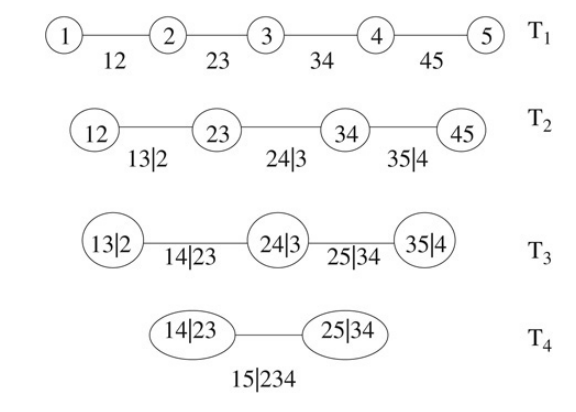
\includegraphics[width = 0.6 \textwidth]{Imagenes/Dvine5var.png}
    \caption{D-vine de 5 variables, 10 aristas y 4 árboles.}
    \label{fig:Dvine5}
\end{figure}

Al finalizar esta construcción, se obtiene una forma sencilla de visualizar la representación de la distribución conjunta utilizando cópulas a pares, como se muestra en la ecuación \eqref{dist5}. Los argumentos de las funciones cópula son distribuciones condicionales, en la ecuación \eqref{distC5} se muestra sus evaluaciones.

\begin{equation}\label{dist5}
     \begin{split}
         f(x_1, x_2, x_3, x_4, x_5) & = f(x_1) \cdot f(x_2) \cdot f(x_3) \cdot f(x_4) \cdot f(x_5)  \\
         & \cdot C_{12} \cdot C_{23} \cdot C_{34} \cdot C_{45} \quad (T_1)\\
         & \cdot C_{13|2} \cdot C_{24|3} \cdot C_{35|4} \quad (T_2)\\\
         & \cdot C_{14|23} \cdot C_{25|34} \quad (T_3)\\
         & \cdot C_{15|234} \quad (T_4)\\
     \end{split}
\end{equation}


\begin{equation}\label{distC5}
     \begin{split}
         f(x_1, x_2, x_3, x_4, x_5) & = f(x_1) \cdot f(x_2) \cdot f(x_3) \cdot f(x_4) \cdot f(x_5)  \\
         & \cdot C_{12}(F_1(x_1), F_2(x_2)) \cdot C_{23}(F_2(x_2), F_3(x_3)) \\
         & \cdot C_{34}(F_3(x_3), F_4(x_4)) \cdot C_{45}(F_4(x_4), F_5(x_5)) \quad (T_1)\\
         & \cdot C_{13|2}(F_{1|2}(x_1|x_2), F_{3|2}(x_3|x_2)) \cdot C_{24|3}(F_{2|3}(x_2|x_3), F_{4|3}(x_4|x_3))\\
         &\cdot C_{35|4}(F_{3|4}(x_3|x_4), F_{5|4}(x_5|x_4)) \quad (T_2)\\
         & \cdot C_{14|23}(F_{1|23}(x_1|x_2, x_3), F_{4|23}(x_4|x_2, x_3)) \\
         & \cdot C_{25|34}(F_{2|34}(x_2|x_3, x_4), F_{5|34}(x_5|x_3, x_4)) \quad (T_3)\\
         & \cdot C_{15|234}(F_{1|234}(x_1|x_2, x_3, x_4), F_{5|234}(x_5|x_2, x_3, x_4)) \quad (T_4)\\
     \end{split}
\end{equation}
  %%%%%%%%%%%%%%%%%%%%%%%%%%%%%%%%%%%%%%%%%%%%%%%%%%%%%%
  %%%%%%%%%%%%%%   R E G R E S I O N   %%%%%%%%%%%%%%%%%
  %%%%%%%%%%%%%%%%%%%%%%%%%%%%%%%%%%%%%%%%%%%%%%%%%%%%%%

\section{Regresión Cuantílica Usando D-Vines}

Como es típico en los métodos de regresión, el objetivo principal es comprender o predecir la variable respuesta $Y$ a partir de las covariables $X_1, X_2, \dots , X_d$.

\begin{equation}\label{regresion}
    y = \Phi_{\alpha}(x)
\end{equation}

Qué es la solución de 

\begin{equation}
     \mathbb{P}[Y \leq y | X_1 = x_1, \dots, X_n = x_n ] = \alpha
\end{equation}

Ejemplo de la solución para una covariable

\begin{equation}
    F_{y|x}(y|x) = \frac{\partial }{\partial u_x} C_{yx}(F_y(y), u_x) \Big|_{u_x = F_x(x)}  
\end{equation}

En general, 

\begin{equation}
    F_{y|\overline{x}}(y|\overline{x}) = \frac{\partial }{\partial u_{\overline{x}}} C_{y\overline{x}}(F_y(y), u_{\overline{x}}) \Big|_{u_{\overline{x}} =F_{\overline{x}(x)}} 
\end{equation}

Ejemplo de regresión con 3 variables 

\begin{equation}
    \begin{aligned}
    C_{V \mid U_1, U_2, U_3}\left(v \mid u_1, u_2, u_3\right) 
    = & h_{V \mid U_3 ; U_1, U_2}\left(C_{V \mid U_1, U_2}\left(v \mid u_1, u_2\right) \mid C_{U_3 \mid U_1, U_2}\left(u_3 \mid u_1, u_2\right)\right) \\
    = & h_{V \mid U_3 ; U_1, U_2}\left(h_{V \mid U_2 ; U_1}\left(C_{V \mid U_1}\left(v \mid u_1\right) \mid C_{U_2 \mid U_1}\left(u_2 \mid u_1\right)\right) \mid\right. \\
    & \left.h_{U_3 \mid U_1 ; U_2}\left(C_{U_3 \mid U_2}\left(u_3 \mid u_2\right) \mid C_{U_1 \mid U_2}\left(u_1 \mid u_2\right)\right)\right) \\ 
    = & h_{V \mid U_3 ; U_1, U_2}\left(h_{V \mid U_2 ; U_1}\left(h_{V \mid U_1}\left(v \mid u_1\right) \mid h_{U_2 \mid U_1}\left(u_2 \mid u_1\right)\right) \mid\right. \\
    & \left.h_{U_3 \mid U_1 ; U_2}\left(h_{U_3 \mid U_2}\left(u_3 \mid u_2\right) \mid h_{U_1 \mid U_2}\left(u_1 \mid u_2\right)\right)\right).
    \end{aligned}
\end{equation}


Después de haber ilustrado el funcionamiento con un pequeño ejemplo de tres variables, el siguiente paso será proporcionar una descripción exhaustiva de la implementación del algoritmo disponible en GitHub \url{https://github.com/BesitosDeBaba/deerVineReg}.

%%%%%%%%%%%%%%%%%%%%%%%%%%%%%%%%%%%%%%%%%%%%%%%%%
%%%%%%%%%% G R A F O  I N I C I A L  %%%%%%5%%%%%
%%%%%%%%%%%%%%%%%%%%%%%%%%%%%%%%%%%%%%%%%%%%%%%%%
\section{Descripción de la Implementación Computacional}

A continuación, se abordarían aspectos como los algoritmos utilizados para el ajuste de cópulas, las técnicas de optimización para la estimación de parámetros y las estrategias para la validación del modelo. 

\subsection{Formación del Grafo Inicial}

El programa ofrece dos opciones para construir el grafo inicial:

\begin{enumerate}
    \item \textbf{Construir el árbol}. Se basa en utilizar la medida de dependencia de $\sigma$ Schweizer y Wolff, en su forma empírica como se mostró en ecuación \eqref{SWEemp}. Por lo tanto, para iniciar el algoritmo, es necesario calcular la matriz que contenga la dependencia $\sigma$ entre todas las variables a la cual se le llamará $\Sigma$.

    En el algoritmo \ref{algT1}, se describe la formación del primer árbol.

    \item \textbf{Especificar el árbol}. La segunda opción consiste en introducir manualmente la secuencia a través del entorno de fórmulas de R, donde se especifica la relación deseada entre las variables. Por ejemplo, $Y \sim x_1 + x_2 + x_3$. Este enfoque se utiliza con el propósito de establecer la relación deseada, especialmente desde un punto de vista médico o  por cuestiones experimentales.
\end{enumerate}

\begin{algorithm}[H]
      \caption{Arból Inicial}
      \label{algT1}
      \begin{algorithmic}[1]  
        \Require{Matriz de dependencia $\Sigma$; número total de variables (contando la variable respuesta) $n$}
        \Ensure{Formación del árbol inicial.}
        
        \State $i = 1$
        \State Asignar al nodo actual la variable respuesta, $Nodo_{actual}$.
        
        \While{$i < N$ \do}
          \State Buscar en la columna o renglón del nodo actual el nodo con la dependencia más alta, llamesé $Nodo_{nuevo}$.
          \State Unir $Nodo_actual$ con $Nodo_{nuevo}$.
          \State Actualizar $Nodo_{actual}$ con $Nodo_{nuevo}$.     
          \State{i=i+1}
        \EndWhile
       
    \State{\textbf{Output:} Devolver el grafo.}
      \end{algorithmic}
    \end{algorithm}

%%%%%%%%%%%%%%%%%%%%%%%%%%%%%%%%%%%%%%%%%%%%%%%%%
%%%%%%%%%%%%%% F O R W A R D  %%%%%%%%%%%%%5%%%%%
%%%%%%%%%%%%%%%%%%%%%%%%%%%%%%%%%%%%%%%%%%%%%%%%%

\subsection{Forward}

El siguiente paso consiste en estimar las cópulas utilizando la función \textit{BiCopSelect}. En este proyecto, nos centraremos exclusivamente en el ajuste de cópulas perimétricas; las razones de esta elección se explicarán en el próximo capítulo. Además, para calcular las funciones de distribución condicionales, o su equivalente, la derivada de cópula como se muestra en la ecuación \eqref{fact}, se utilizará la función \textit{BiCopHfunc2}, ambas disponibles en la biblioteca de R, \textbf{VineCopula} para más detalles de implementación ver \url{https://cran.r-project.org/web/packages/VineCopula/index.html}. Es necesario calcular las funciones $h$ en cada nivel para completar la etapa de avance (forward). Estas funciones $h$ serán necesarias para la etapa de retroceso (backward) y para realizar predicciones precisas.

La transformación a escala $u$ hace referencia a convertir las variables aleatorias marginales en distribuciones uniformes en el intervalo $[0, 1]$, es necesaria para trabajar con cópulas. Se realiza aplicando la función de distribución acumulativa empírica de cada variable aleatoria como se describe en \eqref{fdaEmp}.

Adicionalmente, de acuerdo al paquete \textit{VineCopula}, las cópulas son seleccionadas usando \textit{Akaike} y \textit{Bayesian Information Criteria} (AIC y BIC), los cuales están definidos en las ecuaciones \ref{AIC} y \ref{BIC} respectivamente. Inicialmente, todas las cópulas disponibles se ajustan utilizando la estimación de máxima verosimilitud. Luego, se calculan los criterios para todas las familias de cópulas disponibles y se elige la familia con el valor mínimo.

\begin{equation}\label{AIC}
    AIC := -2 \sum_{i=1}^N \ln[c(u_{i,1},u_{i,2}|\boldsymbol{\theta})] + 2k,
\end{equation}

Donde $k$ es igual a $1$ para cópulas de un parámetro y $k$ es igual a $2$ para cópulas de dos parámetros como las cópulas t-, BB1, BB6, BB7 y BB8.

\begin{equation}\label{BIC}
    BIC := -2 \sum_{i=1}^N \ln[c(u_{i,1},u_{i,2}|\boldsymbol{\theta})] + \ln(N)k.
\end{equation}

Notesé que el BIC penaliza más fuerte a las familias de dos parámetros que el AIC.

En la Algoritmo \ref{algfordward} se describe detalladamente el proceso de ajuste de cada cópula utilizada en la D-vine y en la Figura \ref{fig:construccion} se muestra un diagrama que representa como se ejecuta este ajuste.

\begin{algorithm}[H]
      \caption{Forward}
      \label{algfordward}
      \begin{algorithmic}[1]  
        \Require{Data frame con los observaciones en el orden que dicto el algoritmo anterior, $data$: número de variables $n$.}
        \Ensure{Estimación de las cópulas y las funciones $h$.}

        \State $copulas =  \left [  \right ]$; $hs =  \left [  \right ]$; $niveles = n-1$
        
        \State Obtener la función de distribución empírica de cada variable y posteriormente cada una transfórmala a escala $u$, con su respectiva función de distribución. 
        \State Asignar a $dataU$ los datos en escala $u$.
        
        \State $i = 1$
        \While{$i \leq niveles$ \do}
          \State Estimar cada cópula con la función $BiCopSelect$ de $R$. Para $i = 1$ los argumentos corresponde la datos de $dataU$, para los otros casos corresponden a funciones $h$.
          \State Calcular las funciones $h$ de cada cópula para el siguiente nivel.
          \State Añadir las copulas en $copulas$.
          \State Añadir las funciones $h$ a $hs$.
          \State{i=i+1}
        \EndWhile
       
    \State{\textbf{Output:} Devolver $copulas$ y $hs$.}
      \end{algorithmic}
    \end{algorithm}



Después de realizar el ajuste, como era de esperar, se desea evaluar la existencia de la dependencia modelada. Para determinar si hay independencia entre las variables, es decir, si las cópulas que modelan la dependencia entre ellas pueden simplificarse a la cópula independiente, se emplea la estadística descrita en la ecuación \eqref{T} para realizar el test de independencia implementado en \textbf{VineCopula}.
    
\begin{equation}\label{T}
    T = \sqrt{\frac{9N(N - 1)}{2(2N + 5)}} \times |\hat{\tau}|,
\end{equation}

Donde $N$ es el número de observaciones y $\hat{\tau}$ es el tau de Kendall empírica de los vectores de datos $u_1$ u $u_2$. El valor p de la hipótesis nula de independencia bivariada.

\begin{equation}
    \texttt{p.value} = 2 \times \left(1 - \Phi\left(T\right)\right),
\end{equation}


Donde $\Phi$ es la función de distribución normal estándar.

\begin{figure}[H]
    \centering
    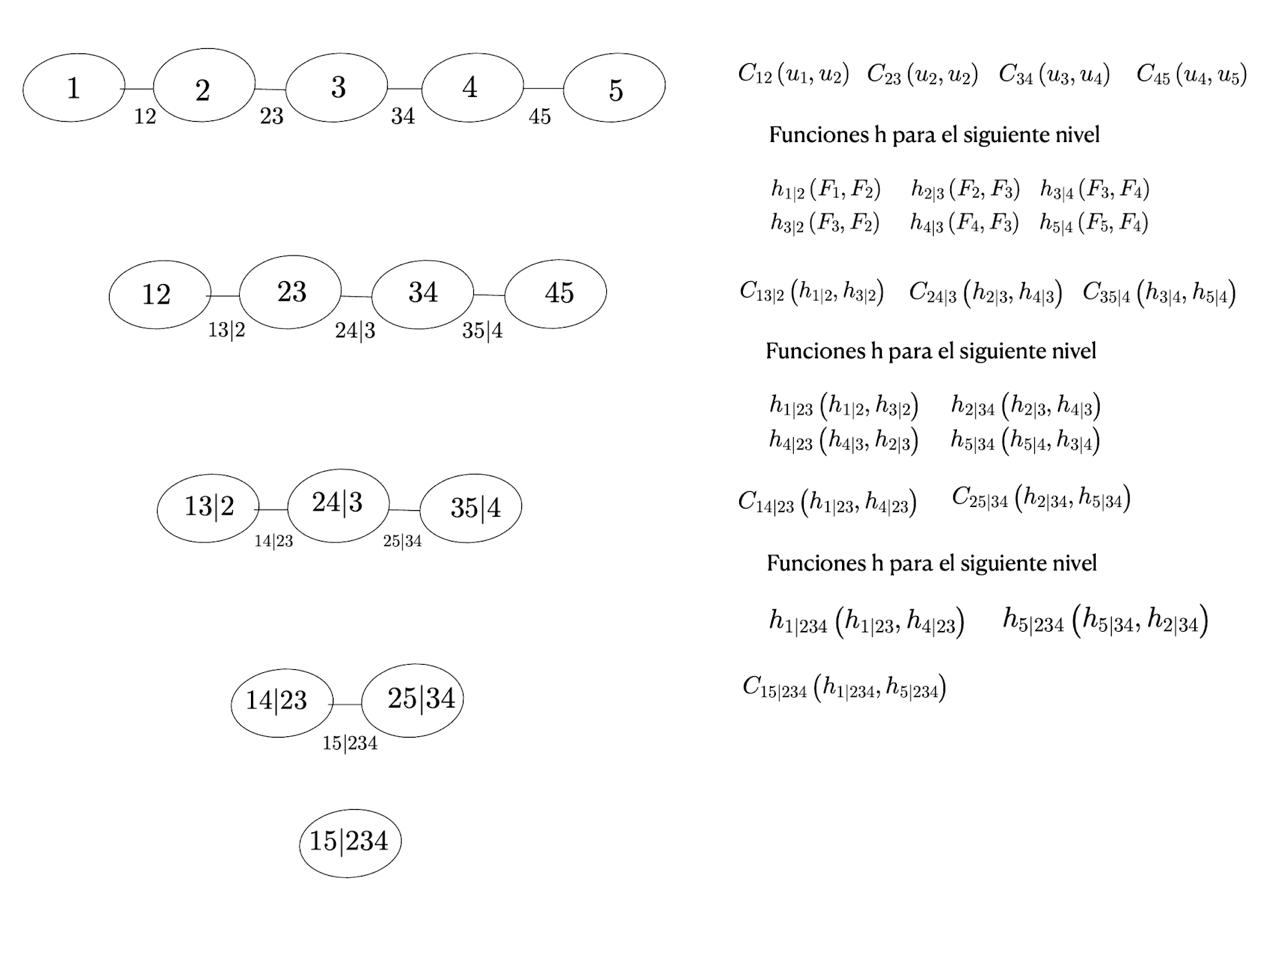
\includegraphics[width = 0.98\textwidth]{Imagenes/Construccion.jpeg}
    \caption{Visualización gráfica para la implementación del modelo D-vine.}
    \label{fig:construccion}
\end{figure}

%%%%%%%%%%%%%%%%%%%%%%%%%%%%%%%%%%%%%%%%%%%%%%%%%
%%%%%%%%%%%%%% F O R W A R D  %%%%%%%%%%%%%5%%%%%
%%%%%%%%%%%%%%%%%%%%%%%%%%%%%%%%%%%%%%%%%%%%%%%%%

\subsection{Backward}

Una vez estimadas las cópulas y las funciones $h$  en cada nivel del árbol de cópulas, Ahora, se tiene que realizar las predicciones sobre las variables aleatorias originales. No hay que olvidar que, hay que obtener las funciones inversas esto se hará usando la función \textit{BiCopHinv2} que viene implementada en la librería \textbf{VineCopula}. Cabe mencionar que el orden de los argumentos es importante ya que obtiene la inversa con respecto a la segunda entrada. Se da en pseudo código en el Algoritmo \ref{algbackward}.


\begin{algorithm}[H]
      \caption{Backward}
      \label{algbackward}
      \begin{algorithmic}[1]  
        \Require{Data frame con los observaciones obtenidas del forward, $dataU$; lista con las funciones $h$ ajustadas en el backward, $hs$ ; lista que contiene las copulas ajustadas en el forward,  $copulas$; nivel de confiabilidad; $\alpha$.}
        \Ensure{Regresión Cuantil.}
        \State{$alphas = rep(alpha, nrows(dataU))$}
        
        \State $i = 1$
        \While{$i \leq niveles$ \do}
          \State Usar $BiCopHinv2$ para cada cópula creada con usando sus respectivas funciones $h$ en la variable $aux$. En la primera iteración los argumentos corresponden al vector $alphas$ y $dataU$.
          \State Actualizar $alphas = aux$
          \State{i=i+1}
        \EndWhile
       
    \State{\textbf{Output:} Devolver $alphas$.}
      \end{algorithmic}
    \end{algorithm}

Al finalizar el proceso descrito, se obtienen las cópulas ajustadas, las cuales son fundamentales cuando se pretende que cualquier individuo pueda ingresar sus datos y recibir un pronóstico preciso. Estas cópulas ajustadas capturan la estructura de dependencia entre las variables de la base dada, lo que permite generar predicciones para nuevas observaciones. 